\subsection{Graphs of Quadratics}
\begin{definition}[Graphing Quadratics]
	The process of drawin a U-shaped curve called a \textit{parabola} on a grid based on an equation where the highest power of the variable is $2$ $(f(x) = ax^2 + bx + c)$.
\end{definition}
\textbf{Note: }The graph will always look like if $a$ is. 
\begin{enumerate}
	\item if $a > 0$ it becomes an upward opening parabola. \\
	\begin{center}
	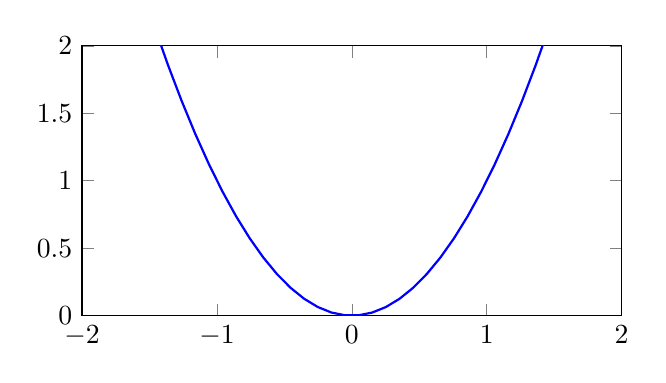
\begin{tikzpicture}
		\begin{axis}[
		    xmin = -2, xmax = 2,
		    ymin = 0, ymax = 2,
		    axis equal image
		]
		    \addplot [domain=-5:5, samples=100, thick, blue] {x^2};
		\end{axis}
	\end{tikzpicture}
	\end{center}
	\item if $a < 0$ it becomes a downward opening parabola. \\
	\begin{center}
	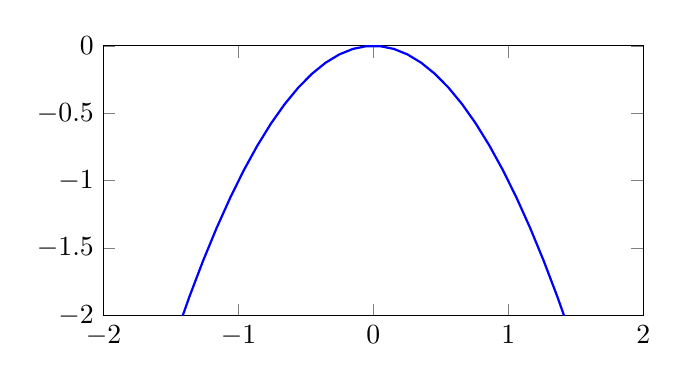
\begin{tikzpicture}
		\begin{axis}[
		    xmin = -2, xmax = 2,
		    ymin = -2, ymax = 0,
		    axis equal image
		]
		    \addplot [domain=-5:5, samples=100, thick, blue] {-(x^2)};
		\end{axis}
	\end{tikzpicture}
	\end{center}
\end{enumerate}

\begin{definition}[$y$ Intercept]
	The point where the graph (a U-shaped curve called a parabola) crosses the vertical $y$-axis, always occuring where $x = 0$. The $y$-intercept is simply the constant number $c$.
	$$(0, c)$$
\end{definition}
\begin{definition}[$x$ Intercept]
	A point where the graph (a U-shaped curve called a parabola) crosses the horizontal $x$-axis.
	$$ax^2 + bx + c = 0$$
\end{definition}
\begin{definition}[Vertex]
	The turning point on a parabola's U-shaped graph where the function reaches its maximum or minimum value, and the graph changes direction.
	$$\left(\frac{b}{2a}, f(x)\right)$$
	Or we can complete the square for the vertex form.
\end{definition}
\begin{example}[Quadratics Graphs]
	\hfill
	\begin{enumerate}
		\item $f(x) = 2x^2 + 8x + 5$
		\begin{enumerate}
			\item Vertex: \\
			$\left(-\frac{(8)}{2(2)}, \quad \right)$ \\
			\textbf{Note: }We plug in $-2$ into the function. \\
			$(-2, -3)$
			\item $y$-intercept: \\
			$(0, 5)$
			\item $x$-intercept: \\
			$2x^2 + 8x + 5 = 0$ \\
			$x = \frac{-(8) \pm \sqrt{(8)^2 - 4 (2)(5)}}{2(2)}$ \\
			$x = \frac{-8 \pm \sqrt{24}}{4}$ \\
			$x \approx -3.22 \land x \approx -0.77$
		\end{enumerate}
		\begin{center}
		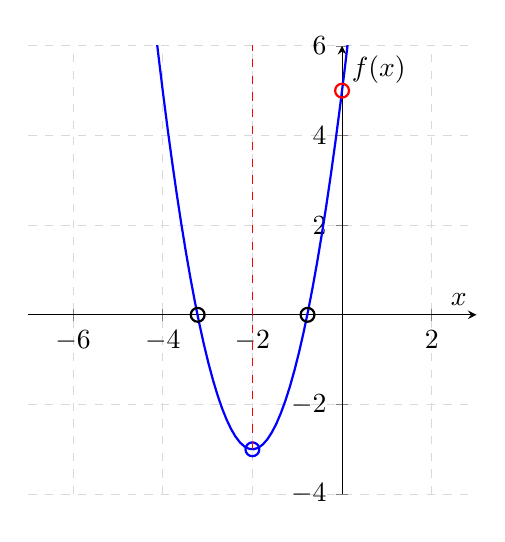
\begin{tikzpicture}
			\begin{axis}[
			    axis lines = center,
			    xlabel = $x$,
			    ylabel = $f(x)$,
			    xmin = -7, xmax = 3,
			    ymin = -4, ymax = 6,
			    grid = major,
			    grid style = {dashed, gray!30},
			    axis equal image
			]
			    \addplot [domain=-5:5, samples=100, thick, blue] {2*x^2+8*x+5};
				\draw[blue, thick] (axis cs:-2,-3) circle (2.5pt);
				\draw[red, thick] (axis cs:0, 5) circle (2.5pt);
				\draw[dashed, red] (axis cs: -2,-3) -- (axis cs:-2,7);
				\draw[black, thick] (axis cs: -3.22, 0) circle (2.5pt);
				\draw[black, thick] (axis cs: -0.77, 0) circle (2.5pt);
			\end{axis}
		\end{tikzpicture}
		\end{center}
	\end{enumerate}
\end{example}
